\documentclass[a4paper,10pt]{article}

\usepackage[utf8]{inputenc}
\usepackage[spanish]{babel}
\usepackage{graphicx}
\usepackage{listings}
\usepackage{appendix}
\usepackage{pdfpages}
\usepackage{fancyhdr}
\usepackage{ulem}
\usepackage{float}
\pagestyle{fancy}

\def\dashuline{\bgroup 
  \ifdim\ULdepth=\maxdimen  % Set depth based on font, if not set already
   \settodepth\ULdepth{(j}\advance\ULdepth.4pt\fi
  \markoverwith{\kern.15em
  \vtop{\kern\ULdepth \hrule width .3em}%
  \kern.15em}\ULon}

\begin{document}

\lhead{\fancyplain{}{Base de Datos 75.15}}
\rhead{\fancyplain{}{Trabajo Pr\'actico Grupal}}

\setcounter{page}{2}

\newpage
\thispagestyle{empty}
\tableofcontents

\newpage
\section{Modelo Entidad Relaci\'on}
  \subsection{Diagrama}
    \begin{center}
      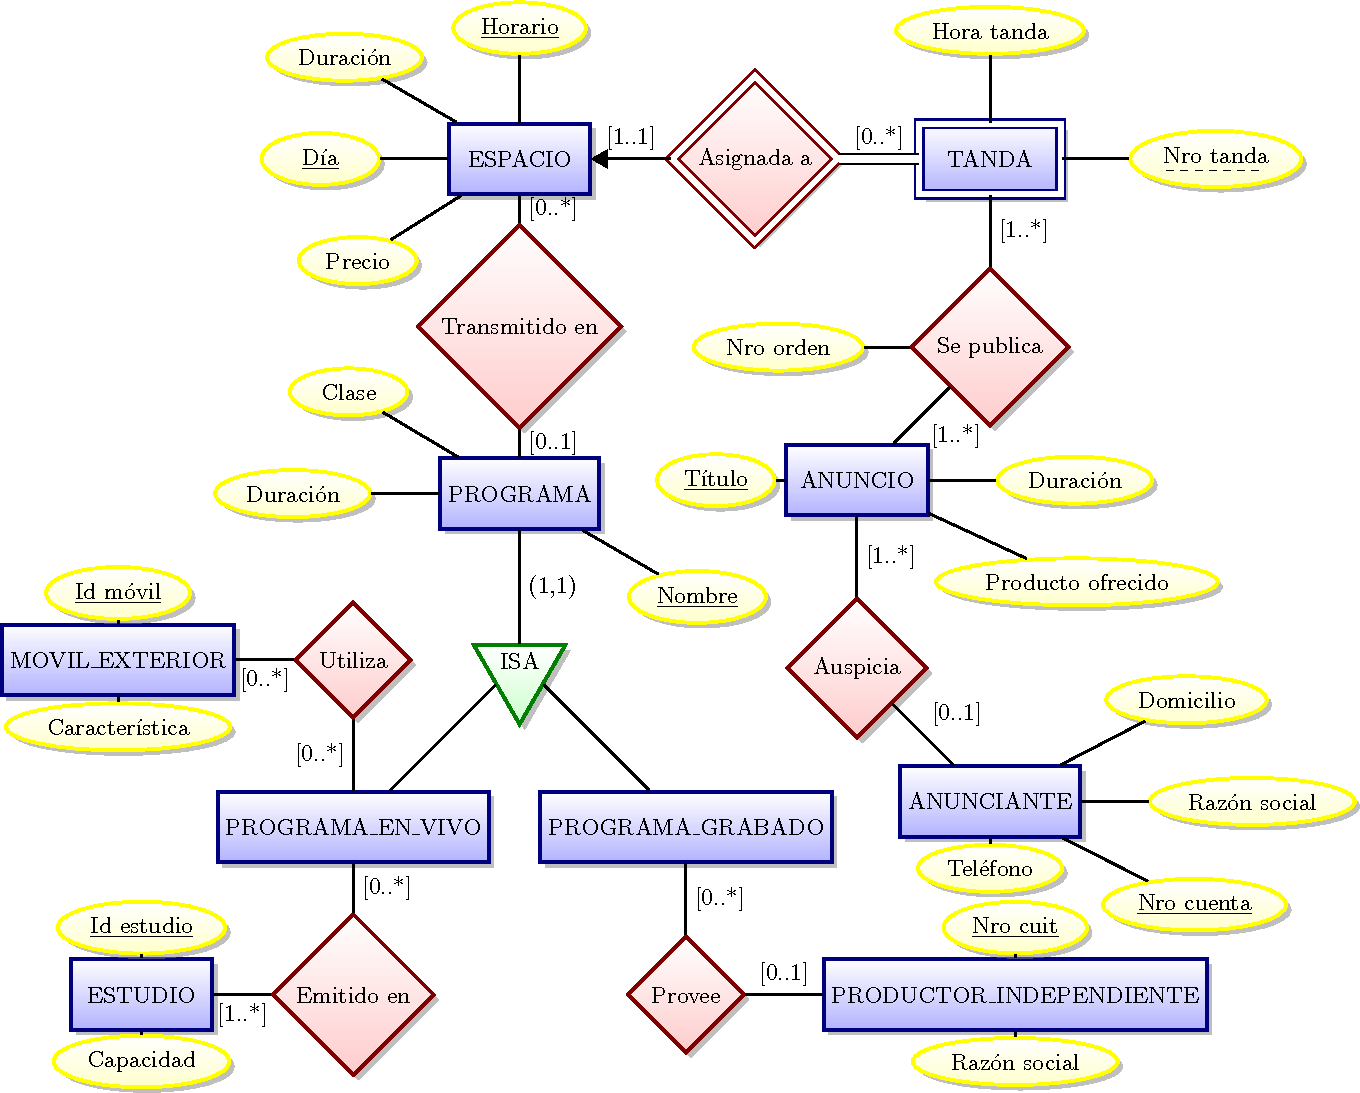
\includegraphics[width=18cm, height=12cm, angle=-90]{ModeloE-R/ModeloE-R.png}   
    \end{center}
  \subsection{Hip\'otesis}
    \begin{enumerate}
      \item Cada m\'ovil de exterior posee un id que lo identifica un\'ivocamente. 
      \item Un programa puede ser en vivo o grabado.
      \item S\'olo los programas en vivo poseen estudios de emisi\'on.
    \end{enumerate}
    
  \subsection{Diccionario}
    \subsubsection{Entidades}
    \begin{flushleft}
      \begin{large} \bf{Espacio} \end{large}
    \end{flushleft}
      \begin{tabular}{| p{2cm} | p{9cm} |}
	\hline
	\multicolumn{2}{|l|}{\bf{Descripci\'on:}} \\
	\hline
	\multicolumn{2}{|l|}{Un espacio es una divisi\'on del horario de transmisi\'on del canal.} \\
	\hline	
	\multicolumn{2}{|l|}{\bf{Especificaci\'on de atributos:}} \\
	\hline
	- D\'ia & El d\'ia en el que se emite el espacio. \\
	\hline \hline
	- Horario & El horario en el que se emite el espacio. \\
	\hline \hline
	- Duraci\'on & La duraci\'on del espacio.\\
	\hline \hline
	- Precio & El precio por segundo en el aire del espacio.\\
	\hline
	\multicolumn{2}{|l|}{\bf{Especificaci\'on de identificador \'unico:}} \\
	\hline
	\multicolumn{2}{|l|}{- D\'ia + Horario} \\
	\hline
      \end{tabular}
    
    \begin{flushleft}
      \begin{large} \bf{Tanda} \end{large}
    \end{flushleft}
      \begin{tabular}{| p{2cm} | p{9cm} |}
	\hline
	\multicolumn{2}{|l|}{\bf{Descripci\'on:}} \\
	\hline
	\multicolumn{2}{|l|}{Un tanda es un espacio donde se publicitan anuncios.} \\
	\hline	
	\multicolumn{2}{|l|}{\bf{Especificaci\'on de atributos:}} \\
	\hline
	- Hora\_tanda & La hora de comienzo de la tanda. \\
	\hline \hline
	- Nro\_tanda & El n\'umero de tanda correspondiente a un programa. \\
	\hline
	\multicolumn{2}{|l|}{\bf{Especificaci\'on de identificador \'unico:}} \\
	\hline
	\multicolumn{2}{|l|}{- D\'ia + Horario + Nro\_tanda} \\
	\hline
      \end{tabular}

    \begin{flushleft}
      \begin{large} \bf{Anuncio} \end{large}
    \end{flushleft}
      \begin{tabular}{| p{2cm} | p{9cm} |}
	\hline
	\multicolumn{2}{|l|}{\bf{Descripci\'on:}} \\
	\hline
	\multicolumn{2}{|l|}{Un anuncio es un espacio, dentro de una tanda, destinado a dar a conocer} \\
	\multicolumn{2}{|l|}{un producto.} \\
	\hline	
	\hline	
	\multicolumn{2}{|l|}{\bf{Especificaci\'on de atributos:}} \\
	\hline
	- T\'itulo & El t\'itulo del anuncio. \\
	\hline \hline
	- Duraci\'on & La duraci\'on del anuncio. \\
	\hline \hline
	- Producto \newline ofrecido & El producto ofrendido del anuncio. \\
	\hline
	\multicolumn{2}{|l|}{\bf{Especificaci\'on de identificador \'unico:}} \\
	\hline
	\multicolumn{2}{|l|}{- T\'itulo} \\
	\hline
      \end{tabular}

    \newpage
    \begin{flushleft}
      \begin{large} \bf{Anunciante} \end{large}
    \end{flushleft}
      \begin{tabular}{| p{2cm} | p{9cm} |}
	\hline
	\multicolumn{2}{|l|}{\bf{Descripci\'on:}} \\
	\hline
	\multicolumn{2}{|l|}{Un anunciante auspicia a lo sumo un producto, mediante un anuncio.} \\
	\hline	
	\multicolumn{2}{|l|}{\bf{Especificaci\'on de atributos:}} \\
	\hline
	- Nro\_cuenta & El n\'umero de cuenta del anunciante. \\
	\hline \hline
	- Domicilio & El domicilio del anunciante. \\
	\hline \hline
	- Raz\'on\_ \newline social & La raz\'on social del anunciante. \\
	\hline \hline
	- Tel\'efono & El tel\'efono del anunciate. \\
	\hline
	\multicolumn{2}{|l|}{\bf{Especificaci\'on de identificador \'unico:}} \\
	\hline
	\multicolumn{2}{|l|}{- Nro\_cuenta} \\
	\hline
      \end{tabular}

    \begin{flushleft}
      \begin{large} \bf{Programa} \end{large}
    \end{flushleft}
      \begin{tabular}{| p{2cm} | p{9cm} |}
	\hline
	\multicolumn{2}{|l|}{\bf{Descripci\'on:}} \\
	\hline
	\multicolumn{2}{|l|}{Un programa es un bloque con contenido que transmitir\'a el canal} \\
	\multicolumn{2}{|l|}{periodicamente} \\
	\hline	
	\multicolumn{2}{|l|}{\bf{Especificaci\'on de atributos:}} \\
	\hline
	- Clase & El tipo de programa que se transmite. \\
	\hline \hline
	- Nombre & Nombre del programa. \\
	\hline \hline
	- Duraci\'on & La duraci\'on del programa.\\
	\hline
	\multicolumn{2}{|l|}{\bf{Especificaci\'on de identificador \'unico:}} \\
	\hline
	\multicolumn{2}{|l|}{- Nombre} \\
	\hline
      \end{tabular}
  
    \begin{flushleft}
      \begin{large} \bf{Programa\_en\_vivo} \end{large}
    \end{flushleft}
      \begin{tabular}{| p{2cm} | p{9cm} |}
	\hline
	\multicolumn{2}{|l|}{\bf{Descripci\'on:}} \\
	\hline
	\multicolumn{2}{|l|}{Un programa en vivo es un programa que se transmite en vivo} \\
	\hline	
	\multicolumn{2}{|l|}{\bf{Especificaci\'on de atributos:}} \\
	\hline
	- No tiene & \\
	\hline
	\multicolumn{2}{|l|}{\bf{Especificaci\'on de identificador \'unico:}} \\
	\hline
	\multicolumn{2}{|l|}{- Hereda la clave de la entidad Programa} \\
	\hline
      \end{tabular} 
  
    \begin{flushleft}
      \begin{large} \bf{Programa\_grabado} \end{large}
    \end{flushleft}
      \begin{tabular}{| p{2cm} | p{9cm} |}
	\hline
	\multicolumn{2}{|l|}{\bf{Descripci\'on:}} \\
	\hline
	\multicolumn{2}{|l|}{Un programa grabado es un programa que se graba y luego se transmite} \\
	\hline	
	\multicolumn{2}{|l|}{\bf{Especificaci\'on de atributos:}} \\
	\hline
	- No tiene & \\
	\hline
	\multicolumn{2}{|l|}{\bf{Especificaci\'on de identificador \'unico:}} \\
	\hline
	\multicolumn{2}{|l|}{- Hereda la clave de la entidad Programa} \\
	\hline
      \end{tabular}

    \newpage
    \begin{flushleft}
      \begin{large} \bf{M\'ovil\_Exterior} \end{large}
    \end{flushleft}
      \begin{tabular}{| p{2cm} | p{9cm} |}
	\hline
	\multicolumn{2}{|l|}{\bf{Descripci\'on:}} \\
	\hline
	\multicolumn{2}{|l|}{Un m\'ovil exterior es un veh\'iculo preparado para usar en la calle durante} \\
	\multicolumn{2}{|l|}{la emisi\'on de programas en vivo} \\	
	\hline	
	\multicolumn{2}{|l|}{\bf{Especificaci\'on de atributos:}} \\
	\hline
	- Id\_movil & Identifica el movil. \\
	\hline \hline
	- Carac- \newline ter\'istica & Descripci\'on de las caracter\'isticas del movil. \\
	\hline
	\multicolumn{2}{|l|}{\bf{Especificaci\'on de identificador \'unico:}} \\
	\hline
	\multicolumn{2}{|l|}{- Id\_m\'ovil} \\
	\hline
      \end{tabular}
      
    \begin{flushleft}
      \begin{large} \bf{Estudio} \end{large}
    \end{flushleft}
      \begin{tabular}{| p{2cm} | p{9cm} |}
	\hline
	\multicolumn{2}{|l|}{\bf{Descripci\'on:}} \\
	\hline
	\multicolumn{2}{|l|}{Un estudio es el lugar donde se toma lugar un programa en vivo} \\
	\hline	
	\multicolumn{2}{|l|}{\bf{Especificaci\'on de atributos:}} \\
	\hline
	- Id\_estudio & Identifica el estudio. \\
	\hline \hline
	- Capacidad & Cantidad de personas que entran en el estudio. \\
	\hline
	\multicolumn{2}{|l|}{\bf{Especificaci\'on de identificador \'unico:}} \\
	\hline
	\multicolumn{2}{|l|}{- Id\_estudio} \\
	\hline
      \end{tabular} 
      
    \begin{flushleft}
      \begin{large} \bf{Productor\_independiente} \end{large}
    \end{flushleft}
      \begin{tabular}{| p{2cm} | p{9cm} |}
	\hline
	\multicolumn{2}{|l|}{\bf{Descripci\'on:}} \\
	\hline
	\multicolumn{2}{|l|}{Un productor independiente es aquel que se graba un programa y lo} \\
	\multicolumn{2}{|l|}{entrega al canal para ser transmitido} \\	
	\hline	
	\multicolumn{2}{|l|}{\bf{Especificaci\'on de atributos:}} \\
	\hline
	- Nro\_cuit & N\'umero de CUIT del productor. \\
	\hline \hline
	- Raz\'on\_ \newline social & Raz\'on social del productor\\
	\hline
	\multicolumn{2}{|l|}{\bf{Especificaci\'on de identificador \'unico:}} \\
	\hline
	\multicolumn{2}{|l|}{- Nro\_cuit} \\
	\hline
      \end{tabular} 
   
   
    \subsubsection{Interrelaciones}
    
    \begin{flushleft}
      \begin{large} \bf{Asignada\_a} \end{large}
    \end{flushleft}
      \begin{tabular}{| p{11.4cm} |}
	\hline
	\bf{Descripci\'on:} \\
	\hline
	Las tandas son asignadas a los espacios en una programaci\'on. Un espacio puede tener asignadas muchas tandas. \\	
	\hline	
	\bf{Especificaci\'on de identificador \'unico:} \\
	\hline
	- D\'ia + Horario + Nro\_tanda \\
	\hline
      \end{tabular} 
   
    \begin{flushleft}
      \begin{large} \bf{Transmitido\_en} \end{large}
    \end{flushleft}
      \begin{tabular}{| p{11.4cm} |}
	\hline
	\bf{Descripci\'on:} \\
	\hline
	Los distintos programas son transmitidos en los diferentes espacios de la programaci\'on. Los programas pueden repetirse, por lo que pueden tener m\'as de un espacio asignado. \\	
	\hline
	\bf{Especificaci\'on de identificador \'unico:} \\
	\hline
	- Horario + D\'ia\\
	\hline
      \end{tabular}
       
    \begin{flushleft}
      \begin{large} \bf{Se\_publica} \end{large}
    \end{flushleft}
      \begin{tabular}{| p{2cm} | p{9cm} |}
	\hline
	\multicolumn{2}{|l|}{\bf{Descripci\'on:}} \\
	\hline
	\multicolumn{2}{|l|}{Durante las tandas son transmitidos los distintos anuncios(publicidad).} \\
	\multicolumn{2}{|l|}{Durante una tanda se pasan varios anuncios. Adem\'as, los anuncios } \\	
	\multicolumn{2}{|l|}{se repiten en varias tandas.} \\
	\hline
	\multicolumn{2}{|l|}{\bf{Especificaci\'on de atributos:}} \\
	\hline
	- Nro\_orden & Orden en que los anuncios se pasan durante una tanda. \\
	\hline
	\multicolumn{2}{|l|}{\bf{Especificaci\'on de identificador \'unico:}} \\
	\hline
	\multicolumn{2}{|l|}{- D\'ia + Horario + Nro\_tanda + Titulo} \\
	\hline
      \end{tabular}

    \begin{flushleft}
      \begin{large} \bf{Auspicia} \end{large}
    \end{flushleft}
      \begin{tabular}{| p{11.4cm} |}
	\hline
	\bf{Descripci\'on:} \\
	\hline
	Los anuncios son auspiciados por los anunciantes. \\
	\hline	
	\bf{Especificaci\'on de identificador \'unico:} \\
	\hline
	- Titulo \\
	\hline
      \end{tabular}

    \begin{flushleft}
      \begin{large} \bf{Utiliza} \end{large}
    \end{flushleft}
      \begin{tabular}{| p{11.4cm} |}
	\hline
	\bf{Descripci\'on:} \\
	\hline
	Para realizar los programas en vivo, los mismos hacen uso de moviles para transmitirlos. Los mismos moviles son reutilizados por diferentes programas. \\
	\hline	
	\bf{Especificaci\'on de identificador \'unico:} \\
	\hline
	- Id\_m\'ovil + Nombre \\
	\hline
      \end{tabular}

    \begin{flushleft}
      \begin{large} \bf{Emitido\_en} \end{large}
    \end{flushleft}
      \begin{tabular}{| p{11.4cm} |}
	\hline
	\bf{Descripci\'on:} \\
	\hline
	Los programas en vivo se llevan a cabo en un estudio(puede que en m\'as de uno). \\	
	\hline
	\bf{Especificaci\'on de identificador \'unico:} \\
	\hline
	- Id\_estudio + Nombre \\
	\hline
      \end{tabular} 
      
    \begin{flushleft}
      \begin{large} \bf{Provee} \end{large}
    \end{flushleft}
      \begin{tabular}{| p{11.4cm} |}
	\hline
	\bf{Descripci\'on:} \\
	\hline
	Los programas grabados que se emiten son provistos por productores ajenos al canal(productore independientes). \\	
	\hline		
	\bf{Especificaci\'on de identificador \'unico:} \\
	\hline
	- Nombre \\
	\hline
      \end{tabular}

\newpage
\section{Transformaci\'on del Modelo E-R a un Modelo Relacional}
  \subsection{Claves candidatas y for\'aneas}
  \begin{flushleft}
  Las claves candidatas est\'an separadas con punto y coma(;). \\
  En claves compuestas los atributos est\'an con coma(,) y encerradas entre par\'entesis. \\
  Las claves for\'aneas son subrayadas con l\'inea punteada. 
  \end{flushleft}
    \begin{itemize}
      \item ESPACIO: (\underline{D\'ia}, \underline{Horario})
      \item PROGRAMA: \underline{Nombre}
      \item TANDA: (\dashuline{\underline{D\'ia}}, \dashuline{\underline{Horario}}, \underline{Nro\_tanda})
      \item SE\_PUBLICA: (\dashuline{\underline{D\'ia}}, \dashuline{\underline{Horario}}, \dashuline{\underline{Nro\_tanda}}, \dashuline{\underline{T\'itulo}})
      \item ANUNCIO: \underline{T\'itulo}, \dashuline{Nro\_cuenta}
      \item ANUNCIANTE: \underline{Nro\_cuenta}; Raz\'on\_social
      \item PROGRAMA\_GRABADO: \underline{Nombre}
      \item PRODUCTOR\_INDEPENDIENTE: \underline{Nro\_cuit}; Raz\'on\_social
      \item PROGRAMA\_EN\_VIVO: \underline{Nombre}
      \item EMITIDO\_EN: (\dashuline{\underline{Nombre}}, \dashuline{\underline{Id\_estudio}})
      \item ESTUDIO: \underline{Id\_estudio}
      \item UTILIZA: \dashuline{(\underline{Nombre}}, \dashuline{\underline{Id\_m\'ovil}})
      \item MOVIL\_EXTERIOR: \underline{Id\_m\'ovil}
    \end{itemize}

  \subsection{Diagrama resultante de la transformaci\'on}
  \begin{flushleft}
    Las claves primarias son subrayadas con l\'inea s\'olida.
  \end{flushleft}

    \begin{flushleft}
      {\bf{ESPACIO}} (\underline{D\'ia}, \underline{Horario}, Duraci\'on, Precio, Nombre)
    \end{flushleft} 
 
    \begin{flushleft}
      {\bf{PROGRAMA}} (\underline{Nombre}, Duraci\'on, Clase)
    \end{flushleft} 

    \begin{flushleft}
      {\bf{TANDA}} (\underline{D\'ia}, \underline{Horario}, \underline{Nro\_tanda}, Hora\_tanda)
    \end{flushleft} 

    \begin{flushleft}
      {\bf{SE\_PUBLICA}} (\underline{D\'ia}, \underline{Horario}, \underline{Nro\_tanda}, \underline{T\'itulo}, Nro\_orden)    
    \end{flushleft}

    \begin{flushleft}
      {\bf{ANUNCIO}} (\underline{T\'itulo}, Duraci\'on, Producto\_ofrecido, Nro\_cuenta)
    \end{flushleft}

    \begin{flushleft}
      {\bf{ANUNCIANTE}} (\underline{Nro\_cuenta}, Raz\'on\_social, Tel\'efono, Domicilio)
    \end{flushleft}

    \begin{flushleft}
      {\bf{PROGRAMA\_GRABADO}} (\underline{Nombre}, Nro\_cuit)
    \end{flushleft}
   
    \begin{flushleft}
      {\bf{PRODUCTOR\_INDEPENDIENTE}} (\underline{Nro\_cuit}, Raz\'on\_social)
    \end{flushleft}
  
    \begin{flushleft}
      {\bf{PROGRAMA\_EN\_VIVO}} (\underline{Nombre})
    \end{flushleft}

    \begin{flushleft}
      {\bf{EMITIDO\_EN}} (\underline{Nombre}, \underline{Id\_estudio})
    \end{flushleft}
  
    \begin{flushleft}
      {\bf{ESTUDIO}} (\underline{Id\_estudio}, Capacidad)
    \end{flushleft}
  
    \begin{flushleft}
      {\bf{UTILIZA}} (\underline{Nombre}, \underline{Id\_m\'ovil})
    \end{flushleft}
  
    \begin{flushleft}
      {\bf{MOVIL\_EXTERIOR}} (\underline{Id\_m\'ovil}, Caracter\'istica)
    \end{flushleft}

  \subsection{Atributos que pueden tomar valores nulos}
    \begin{flushleft}
      El Modelo Relacional tiene dos restricciones inherentes o impl\'icitas que refieren a las claves primarias y a las claves for\'aneas, llamadas reglas de integridad: 
    \end{flushleft}

    \begin{enumerate}
    \item REGLA DE INTEGRIDAD DE ENTIDAD: Los valores que forman parte de un clave primaria deben estar bien definidos.
    \item REGLA DE INTEGRIDAD REFERENCIAL: Los valores que toman una clave for\'anea deben ser o bien totalmente desconocidos o de lo contrario deben estar defenidos en la relaci\'on donde son clave primaria. 
    \end{enumerate}

    \begin{flushleft}
      A partir de esto \'ultimo, se puede definir que atributos pueden ser nulos.
    \end{flushleft}

    \begin{itemize}
      \item ESPACIO: Duraci\'on, Precio y Nombre.
      \item PROGRAMA: Duraci\'on y Clase.
      \item TANDA: Hora\_tanda.
      \item SE\_PUBLICA: Hora\_tanda y Nro\_orden.
      \item ANUNCIO: Duraci\'on, Producto\_ofrecido y Nro\_cuenta.
      \item ANUNCIANTE: Raz\'on\_social, Tel\'efono y Domicilio.
      \item PROGRAMA\_GRABADO: Nro\_cuit.
      \item PRODUCTOR\_INDEPENDIENTE: Raz\'on\_social.
      \item PROGRAMA\_EN\_VIVO: Ninguno.
      \item EMITIDO\_EN: Ninguno.
      \item ESTUDIO: Capacidad.
      \item UTILIZA: Ninguno.
      \item MOVIL\_EXTERIOR: Caracter\'istica.
    \end{itemize}
    
  \subsection{Diagrama de Modelos de tabla}  
		\begin{figure}[H]
			\begin{center}
				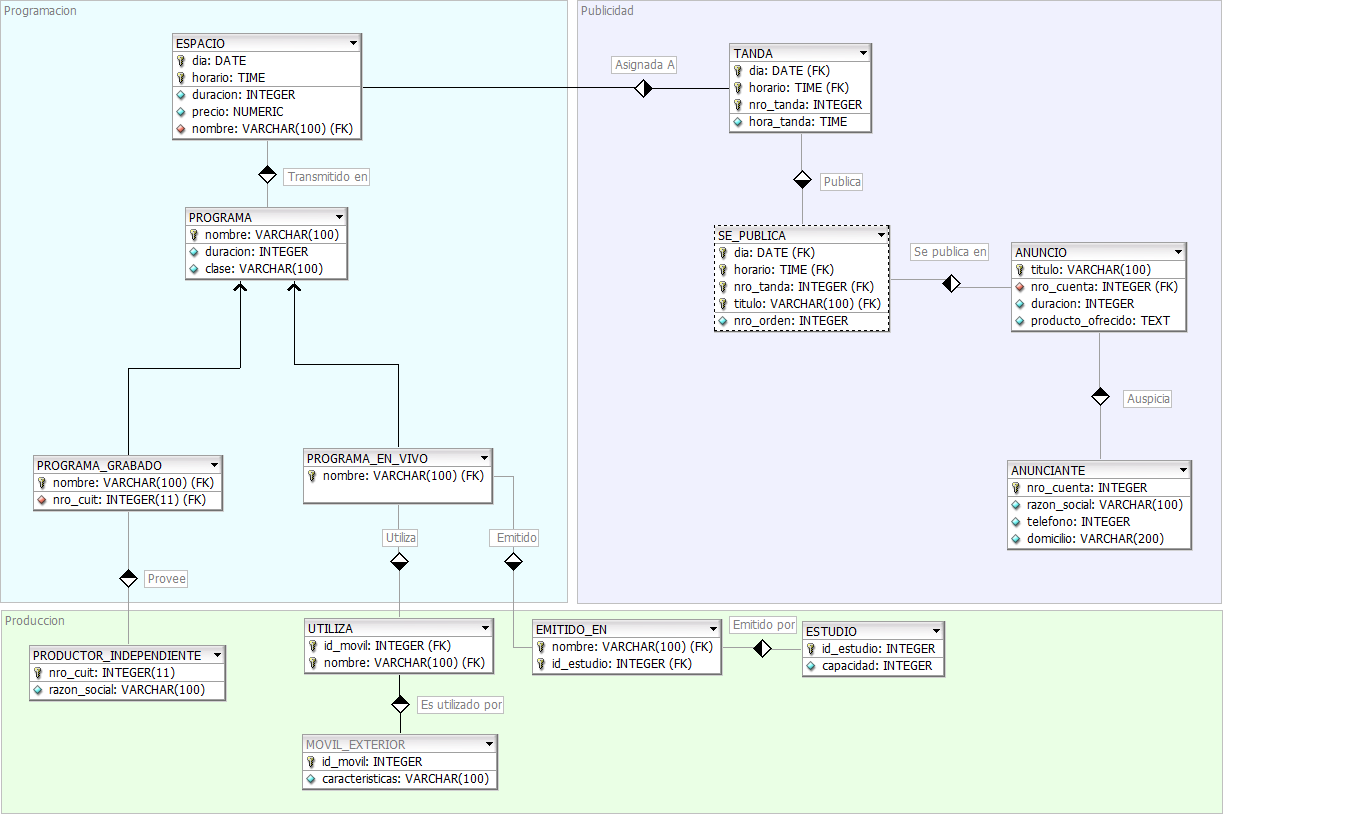
\includegraphics[scale=0.35]{der.png}
				\caption{Diagrama de modelos de tabla}
				\label{fig:flujos}
			\end{center}
		\end{figure}
		
		\begin{flushleft}
    	Algunas alternativas al diagrama presentado que se podr\'ian plantear son:
    \end{flushleft}  
    
    \begin{itemize}
    	\item Para las relaciones cuya cardinalidad \textbf{no} es N:N (ejemplo 1:N), se podr\'ia utilizar una tabla (como en el caso del N:N) esto tiene sus ventajas y desventajas respecto al modelo planteado. La ventaja es que resolver el problema as\'i posibilita llegado el caso cambiar la cardinalidad de la relaci\'on a N:N sin mayores complicaciones. La desventaja es que esta configuraci\'on requiere una tabla m\'as y todo el esfuerzo que implica mantener esa tabla.
    	\item Para el caso particular del atributo Clase en la relaci\'on PROGRAMA, se podr\'ia usar una tabla que tenga como atributos la clase y un c\'odigo \'unico que la identifique y que almacene las diferentes clases de programas. Finalmente a la tabla PROGRAMA se la relaciona con la tabla CLASE por medio del atributo \textit{codigoclase} que se agregar\'ia en la tabla PROGRAMA (ser\'ia una clave for\'anea).
    	Se elegi\'o esta soluci\'on para mantener la simplicidad del modelo de entidad-relaci\'on.
    \end{itemize}
    
\newpage
\section{Consultas SQL}

% Configuración de paquete listings para SQL y tipografia courier.
\lstset{basicstyle=\fontfamily{pcr}\small, language=SQL}

\subsection*{1. \normalsize{Todos los programas que no se emiten los fines de semana.}}

\subsubsection*{Consulta}
\begin{lstlisting} 
select * from programa
where cod_prog not in (select cod_prog from espacio 
                       where dia in ('SAB', 'DOM'))
\end{lstlisting}

\subsubsection*{Resultados}
\begin{tabular}{|l|l|l|l|}
  \hline
    \bf{COD\_PROG} & \bf{NOMBRE} & \bf{CLASE} & \bf{DURACION} \\ 
  \hline
    C22 & Canal ``ETA'' & Humor & 1800 \\ 
  \hline
\end{tabular} 

\subsection*{2. \normalsize{El o los d\'ias de la semana en que el anunciante ``Juan Uncio'', anuncie su mayor cantidad diaria de anuncios.}}

\subsubsection*{Consulta}
\begin{lstlisting}
select dia 
from publicidad p, anuncio a, anunciante e
where p.titulo = a.titulo and 
      a.cuenta = e.cuenta and 
      razon_social = 'Juan Uncio'
group by dia
having count(1) >= all (select count(1)
                        from publicidad p, anuncio a, anunciante e
                        where p.titulo = a.titulo and 
                              a.cuenta = e.cuenta and
                              razon_social = 'Juan Uncio'
                        group by dia)
\end{lstlisting}

\subsubsection*{Resultados}
\begin{tabular}{|l|}
  \hline
    \bf{DIA} \\ 
  \hline
    MAR \\ 
  \hline
\end{tabular} 

\subsubsection*{Comentarios}

Las cl\'ausulas \lstinline|from|, \lstinline|where| y \lstinline|group by| son id\'enticas en ambos selects. En el select principal se obtienen los d\'ias en los que el anunciante ``Juan Uncio'' publica alg\'un anuncio, y en la cl\'ausula \lstinline|having| de \'este se compara la cantidad de anuncios por d\'ia contra su m\'aximo de anuncios por d\'ia. \\

La repetici\'on de c\'odigo (y la consiguiente dificultad para entenderlo/mantenerlo) podr\'ia evitarse usando una vista SQL:

\begin{lstlisting}
create view anuncios_por_dia_juan_uncio(dia, cantidad) as
select dia, count(1)
from publicidad p, anuncio a, anunciante e
where p.titulo = a.titulo and a.cuenta = e.cuenta and 
      razon_social = 'Juan Uncio'
group by dia;

select dia from anuncios_por_dia_juan_uncio
where cantidad = (select max(cantidad) from anuncios_por_dia_juan_uncio);
\end{lstlisting}

Pero esto, a su vez, pordr\'ia ser problem\'atico, ya que se estar\'ia creando una vista adicional en la base de datos que es de inter\'es s\'olo a una consulta particular. Adoptar esta metodolog\'ia para resolver todas las consultas complejas no ser\'ia una soluci\'on pr\'actica escalable, ya que pronto la base de datos se transformar\'ia en un conjunto de much\'isimas vistas poco reutilizables que, si bien no son costosas en t\'erminos de espacio f\'isico como las tablas, agregar\'ian complejidad innecesaria. \\

Lo ideal para no repetir el c\'odigo ser\'ia poder guardar una tabla como una variable temporal, que se descarte luego de salir del \'ambito en que se use. Desgraciadamente esta funcionalidad, m\'as procedural/imperativa, est\'a fuera del estandard SQL, que es m\'as bien un lenguaje declarativo. Algunas extensiones al lenguaje, como PSQL, proveen esta funcionalidad en forma de tablas temporales o variables locales a funciones.

\subsection*{3. \normalsize{La raz\'on social de los anunciantes que anuncian en la mayor cantidad de programas distintos.}}

\subsubsection*{Consulta}
\begin{lstlisting} 
select a.razon_social
from anunciante a, anuncio an, publicidad p, espacio e
where a.cuenta = an.cuenta and an.titulo = p.titulo and 
      p.dia = e.dia and p.hora = e.hora
group by a.razon_social
having count(distinct e.cod_prog) >= all 
       (select count(distinct e.cod_prog)
        from anunciante a, anuncio an, publicidad p, espacio e
        where a.cuenta = an.cuenta and an.titulo = p.titulo and 
              p.dia = e.dia and p.hora = e.hora
        group by a.razon_social)
\end{lstlisting}

\subsubsection*{Resultados}
\begin{tabular}{|l|}
  \hline
    \bf{RAZON\_SOCIAL} \\ 
  \hline
    Ricardo Perez \\
    Juan Uncio \\ 
  \hline
\end{tabular} 

\subsubsection*{Comentarios}
Al igual que en la consulta 2, esta podr\'ia En \'este ejemplo tambi\'en se podr\'ia evitar repetici\'on de c\'odigo usando una vista SQL:

\begin{lstlisting} 
create view programas_por_anunciante(razon_social, programas) as
select razon_social, count(distinct e.cod_prog)
from anunciante a, anuncio an, publicidad p, espacio e
where a.cuenta = an.cuenta and an.titulo = p.titulo and 
      p.dia = e.dia and p.hora = e.hora
group by a.razon_social;

select razon_social from programas_por_anunciante
where programas = (select max(programas) from programas_por_anunciante);

\end{lstlisting}

\subsection*{4. \normalsize{El nombre de los programas grabados que se emitan en promedio m\'as veces por d\'ia los fines de semana que los d\'ias laborales (lunes a viernes).}}

\subsubsection*{Consulta}
\begin{lstlisting} 
select nombre from programa p
where cod_prog in (select cod_prog from produccion) and
      (select count(*) from espacio
       where cod_prog = p.cod_prog and dia in ('SAB', 'DOM')) / 2 
         >
      (select count(*) from espacio
       where cod_prog = p.cod_prog and dia not in ('SAB', 'DOM')) / 5
\end{lstlisting}

\subsubsection*{Resultados}
\begin{tabular}{|l|}
  \hline
    \bf{NOMBRE} \\ 
  \hline
    La Aventura del Punto \\ 
  \hline
\end{tabular} 


\subsubsection*{Suposici\'on}
Los programas grabados son los que tienen una producci\'on asociada. \\

\subsubsection*{Comentarios}
En el primer subquery se cuenta la cantidad de veces que se transmite el programa los fines de semana, y el segundo la cantidad de veces que se transmite los d\'ias de semana. El promedio se saca haciendo una divisi\'on por la cantidad de d\'ias en cada caso, y luego s\'olo se comparan los promedios.


\subsection*{5. \normalsize{El d\'ia, hora y n\'umero de tanda de las tandas que tengan una cantidad de anuncios mayor que el promedio de anuncios por tanda del mismo d\'ia.}}

\subsubsection*{Consulta}
\begin{lstlisting} 
select dia, hora, tanda
from publicidad p
group by dia, hora, tanda
having count(distinct titulo) > (select avg(count(distinct titulo))
                                 from publicidad
                                 where dia = p.dia
                                 group by dia, hora, tanda)
\end{lstlisting}

O bien, calculando el promedio \textit{a mano}:
\begin{lstlisting}
select dia, hora, tanda
from publicidad p
group by dia, hora, tanda
having count(distinct titulo) > (select count(1) from publicidad 
                                 where dia = p.dia) /
                                (select count(1) from tanda
                                 where dia = p.dia)
\end{lstlisting}

O bien, seleccionando directamente de la tabla \lstinline|tanda|:
\begin{lstlisting}
select * from tanda t
where (select count (distinct titulo) from publicidad 
       where dia = t.dia and hora = t.hora and tanda = t.tanda) 
         > 
      (select count(1) from publicidad where dia = t.dia) /
      (select count(1) from tanda where dia = t.dia)
\end{lstlisting}

\subsubsection*{Resultados}
\begin{tabular}{|l|l|l|}
  \hline
    \bf{DIA} & \bf{HORA} & \bf{TANDA} \\ 
  \hline
    DOM & 13:00 & 1 \\
    DOM & 13:00 & 2 \\
    SAB & 11:00 & 1 \\
    SAB & 13:00 & 2 \\
  \hline
\end{tabular} 

\subsubsection*{Suposici\'on}
El enunciado dice ``...las tandas que tengan una cantidad de anuncios...'', con lo cual se supone que lo que se desea tener en cuenta es la cantidad de anuncios distintos en esa tanda, y no la cantidad de publicidades. e.g: si una tanda tiene 3 publicidades, pero las 3 son del mismo anuncio (un lavaje de cerebro importante), se contaría un sólo anuncio en esa tanda. \\

Si lo que se quería era contar la cantidad de publicidades en una tanda, sin importar que se tratara de anuncios repetidos, basta con reemplazar los ``\lstinline|distinct titulo|'' por \lstinline|*| o \lstinline|1| (en cualquiera de las consultas).

\subsubsection*{Comentarios}
Esta consulta es un ejemplo de que ocurre a menudo con SQL: existen muchas formas de obtener la misma información. La elección de la consulta podrá depender de lo que el programador considere más expresivo, o podrían llevarse a cabo pruebas de performance para averiguar cuál es la más conveniente. \\

En este caso, se considera que la forma más expresiva de calcular el promedio de anuncios por tanda de un día dado es la usada en la primer consulta. Pero es posible que la expresión ``\lstinline|avg(count(distinct titulo))|'' no sea soportada por todos los motores de bases de datos, y se tenga que recurrir a calcular el promedio \textit{a mano} como en la segunda o tercer consulta.


\subsection*{6. \normalsize{Para cada d\'ia, mostrar el d\'ia, la hora y el nombre del programa que se emite en el espacio con la mayor cantidad de anuncios distintos de cada d\'ia.}}

\subsubsection*{Consulta}
\begin{lstlisting} 
select e.dia, e.hora, nombre
from espacio e, programa pr, publicidad pu
where e.cod_prog = pr.cod_prog and 
      e.dia = pu.dia and e.hora = pu.hora
group by e.dia, e.hora, nombre
having count(distinct titulo) >= all (select count(distinct titulo) 
                                      from publicidad 
                                      where dia = e.dia 
                                      group by dia, hora)
order by e.dia, e.hora
\end{lstlisting}

\subsubsection*{Resultados}
\begin{tabular}{|l|l|l|}
  \hline
    \bf{DIA} & \bf{HORA} & \bf{NOMBRE} \\ 
  \hline
    DOM & 13:00 & Su Ojo en la Lupa \\ 
    JUE & 11:00 & Viva la Patria \\ 
    JUE & 13:00 & Canal ``ETA'' \\ 
    JUE & 15:00 & Viva la Patria \\ 
    LUN & 11:00 & La Aventura del Punto \\ 
    LUN & 13:00 & Canal ``ETA'' \\ 
    LUN & 15:00 & Viva la Patria \\ 
    MAR & 11:00 & La Aventura del Punto \\ 
    MAR & 13:00 & Canal ``ETA'' \\ 
    MAR & 15:00 & Viva la Patria \\ 
    MIE & 11:00 & La Aventura del Punto \\ 
    MIE & 13:00 & Canal ``ETA'' \\ 
    MIE & 15:00 & Viva la Patria \\ 
    SAB & 13:00 & Su Ojo en la Lupa \\ 
    VIE & 11:00 & Viva la Patria \\ 
    VIE & 13:00 & Su Ojo en la Lupa \\ 
    VIE & 15:00 & Viva la Patria \\ 
  \hline
\end{tabular} 

\subsubsection*{Comentarios}
Como puede existir más de un espacio con la mayor cantidad de anuncios distintos por día, aparecen múltiples resultados para algunos de los días de la semana.

\subsection*{7. \normalsize{El nombre de los programas en vivo que se emiten en todos los d\'ias h\'abiles (lunes a viernes).}}

\subsubsection*{Consulta}
\begin{lstlisting} 
select nombre 
from programa p
where cod_prog not in (select cod_prog from produccion) and
      not exists (select dia from espacio 
                  where dia  in ('LUN', 'MAR', 'MIE', 'JUE', 'VIE') 
                    minus
                  select dia from espacio 
                  where cod_prog = p.cod_prog)
\end{lstlisting}

O bien:

\begin{lstlisting} 
select nombre 
from programa p
where cod_prog not in (select cod_prog from produccion) and
      not exists (select dia from espacio e
                  where dia in ('LUN', 'MAR', 'MIE', 'JUE', 'VIE') 
                        and not exists (select * from espacio 
                                        where cod_prog = p.cod_prog 
                                              and dia  = e.dia))
\end{lstlisting} 

\subsubsection*{Resultados}
\begin{tabular}{|l|}
  \hline
    \bf{NOMBRE} \\ 
  \hline
    Su Ojo en la Lupa \\ 
  \hline
\end{tabular} 

\subsubsection*{Suposiciones}
Los programas en vivo son los no grabados, es decir, los que no tienen una producción asociada. \\

Existe al menos un espacio en cada día de la semana. \\

\subsubsection*{Comentarios}
Esta consulta es tipo una división del álgebra relacional. La consulta con los dos \lstinline|not exists| anidados es correcta, pero la primera resulta más entendible, ya que hay menos anidamiento de selects. La consulta puede \textit{leerse}, en ambos casos, como ``Los programas en vivo tal que no exista día hábil en que el programa no se transmita''. \\

La segunda suposición es necesaria puesto que no existe una tabla de donde se puedan sacar los nombres de los día de la semana. Ni tampoco es posible crear una tabla temporal que los contenga. Ni tampoco, auqnue en teoría es posible\cite{values_expression}, el gestor de base de datos que utiliza el sistema de pruebas permite utilizar una expresión \lstinline|values| para crear una tabla constante:

\begin{lstlisting} 
-- Los dias habiles en que no se transmite el programa p.
select * from (values 'LUN', 'MAR', 'MIE', 'JUE', 'VIE') as habiles
  minus
select dia from espacio where cod_prog = p.cod_prog
\end{lstlisting}

\subsection*{8. \normalsize{Los d\'ias en que se ocupan todos los estudios.}}

\subsubsection*{Consulta}
\begin{lstlisting} 
select distinct dia from espacio e
where not exists (select estudio from estudio
                    minus
                  select estudio 
                  from espacio es, ocupacion o
                  where es.cod_prog = o.cod_prog and es.dia = e.dia)
\end{lstlisting}

\subsubsection*{Resultados}
\begin{tabular}{|l|}
  \hline
    \bf{DIA} \\ 
  \hline
    JUE \\
    LUN \\
    MAR \\
    MIE \\
  \hline
\end{tabular} 

\subsection*{9. \normalsize{La raz\'on social de los anunciantes que tienen al menos un anuncio de sus productos en las emisiones de todos los programas del productor ``ROMUALDO''.}}

\subsubsection*{Consulta}
\begin{lstlisting} 

\end{lstlisting}

\subsubsection*{Resultados}
\begin{tabular}{|l|l|}
  \hline
    \bf{CAMPO1} & \bf{CAMPO2} \\ 
  \hline
    c11 & c21 \\ 
    c21 & c22 \\
  \hline
\end{tabular} 

\subsection*{10. \normalsize{El nombre de los programas que se emiten en todos los d\'ias en que al menos una vez sean utilizados todos los m\'oviles por cualquiera de los programas emitidos en ese d\'ia.}}

\subsubsection*{Consulta}
\begin{lstlisting} 

\end{lstlisting}

\subsubsection*{Resultados}
\begin{tabular}{|l|l|}
  \hline
    \bf{CAMPO1} & \bf{CAMPO2} \\ 
  \hline
    c11 & c21 \\ 
    c21 & c22 \\
  \hline
\end{tabular} 



% Bibliografía.    
\begin{thebibliography}{9}

\bibitem{values_expression}
  \emph{Values Expression}
  \begin{itemize}
    \item http://www.postgresql.org/docs/current/static/sql-values.html 
    \item http://db.apache.org/derby/docs/10.5/ref/rrefsqlj11277.html 
    \item http://it.toolbox.com/blogs/db2luw/sql-you-can-really-use-the-value-of-the-values-clause-12496 
  \end{itemize}

\end{thebibliography}


%APENDICES
\appendix
\newpage
\section{Enunciado}
  
\includepdf[pages=1-2, scale=0.8, pagecommand={\thispagestyle{plain}}]{EnunciadoBD.pdf}
  
  



\end{document}
